\begin{section}{Overview}

Matter exists in many different phases.  These phases can be thought of as the states of matter, each with distinctive properties.  For example, fluids can exist in the vapor, liquid, or solid state.  Transitions between phases can be characterized by how the properties of the matter quantitatively change while transitioning between phases.  For a fluid, the property of interest is density, and it is discontinuous when transitioning between liquid and vapor phases while below the critical point.  When the property of interest is discontinuous while transitioning between phases, it is described as a $1^{st}$ order phase transition.  Phase transitions that involve a continuous behavior of a property are $2^{nd}$ order phase transitions, such as density for supercritical fluids.  Of interest here, is to be able to accurately describe the liquid-vapor phase coexistence curve as shown by the cyan curve in figure (INSERT FIG REF HERE).  


\begin{figure}[H]
	\centering
	\includegraphics[scale=0.5]{p_vs_t_h20.png}
	\caption{Shown above is a typical pressure vs temperature curve for $H_2O$.  The liquid-vapor coexistence curve is shown in cyan, which starts from the triple point in purple and terminates at the critical point in red. }
	\label{fig:p_vs_t_h20}
\end{figure}


In this chapter, I hope to provide sufficient general motivation to help clarify why anyone would consider applying computational statistical physics to predict phase coexistence curves.  I then introduce how some basic models are used when attempting to determine these phase coexistence curves.  While highlighting the early models, I hope to illustrate the underlying shortcoming of them.  This will lead us into chapter $2$ which will focus explaining the details and limitations of Statistical non-Associating Fluid Theory (SnAFT).  Chapter $3$ will introduce how Generalized Renormalization Group Theory (GRGT) can be used in conjunction with SnAFT to overcome the limitations of previous models.  In chapter $4$ I will present my computational code along with pretty figures and results that will highlight much of what was discussed in previous chapters.  Chapter $5$ will be a reflection and discussion of my research with hints as to what can be done going forward.

\end{section}


\begin{section}{Motivation}

The chemical industry relies on accurate predictions of phase coexistence for fluids in order to ensure safe, efficient, and profitable operations.  Models predicting phase coexistence far from criticality have been well established for over a century [REFERENCE?].  More recently it has been of interest to accurately predict phase coexistence near the critical point of fluids because of the useful applications of supercritical fluids.  Our everyday experience with supercritical fluids is limited if not seemingly non-existent.  However, the use of supercritical fluids spans a vast majority of applications directly and indirectly related to our lives.  For instance, super critical carbon dioxide is a non-toxic replacement for the conventional tetrachloroethylene used for dry cleaning.  Supercritical carbon dioxide is also used in the decaffeination process of coffee beans.  For both examples, the pure supercritical fluid is used because of its miscibility.  Carbon dioxide enhanced oil recovery also utilizes this miscible property of the supercriticial fluid.  The process of the oil recovery results in a complicated mixture of fluids all under extreme pressures and temperatures.  Thus the supercritical fluid is no longer a pure fluid.           

For both pure fluids and mixtures, phase coexistence curves can be readily found through experiments focusing on macroscopic quantities like pressure, temperature, and density.  Consider radiator fluid, a mixture, which contains both water and ethylene glycol.  It can be shown experimentally that the phase coexistence depends on the ratio of the water to ethylene glycol in radiator fluid.  If the radiator fluid was mixed at a different ratio of water to ethylene glycol, another experiment must be done in order to find this new mixture's phase coexistence curves.  What if we did yet another ratio of water to ethylene glycol?  Many experiments would need to be done in order to get a wide range of ratios.  On the other had, we can do one experiment at a fixed ratio of water and ethylene glycol, then use information about this experiment to computationally determine what will happen at all ratios.  Basically the computational model depends on arbitrary parameters which can be fit empirically to recreate the phase coexistence at the fixed ratio which the experiment was carried out.  These parameters can then be used to find the phase coexistence at all ratios.  The benefit to this method is that the phase coexistence of mixtures can be explored for a near continuum of ratios, compared to the discrete nature of using only experiments to determine phase coexistence curves. 

It should be noted that simulations can also predict phase coexistence curves just as well as actual experiments for a wide variety of fluids.  The simulations are of two overarching categories; molecular dynamics, and Monte Carlo methods.  Molecular dynamics uses equations of motion for each molecule to collect information about thermodynamic properties.  Monte Carlo methods also extract thermodynamic properties by looking at the changes in energy that could occur if the fluid configuration is altered by moving a single molecule within the system.  With only a few hundred molecules in a system, both molecular dynamics and Monte Carlo methods can produce accurate results of phase coexistence far from the critical point.  In theory, both could accurately describe phase coexistence near the critical point if enough molecules are incorporated into the simulations.  As it turn out, increasing the number of molecules to a sufficient number, to incorporate near critical point information, dramatically affects the time it takes to run the simulations.  The time becomes on the order of somewhere between, not practical and ridiculous.

Computational statistical physics bridges the gap between experiment and simulations, by incorporating relevant physical models in conjunction with statistical thermodynamics to describe fluid properties.  This allows us to come up with clever models, which have physical significance, that can better describe fluid behavior near the critical point in computation time that is feasible.            


\end{section}




\begin{section}{Model}

Phase coexistence inherently depends on the model used.  For example the ideal gas equation of state predicts a gas all the way down to absolute zero.  The ideal gas has the familiar form:

\begin{equation}
pV=Nk_bT
\end{equation}

  This clearly is wrong since oxygen condenses to a liquid at roughly 90K.  The first model with the ability to predict phase coexistence was the van der Waals equation of state, which has the form:
  
\begin{equation}
\left( p + \left( \frac{N}{N_A} \right)^2 \frac{a}{V^2} \right) \left( V - \frac{N}{N_A}  b \right) = N k_B T
\end{equation} 

The van der Waals equation of state is considered to be a cubic equation of state, since expanding it leads to a lingering $V^3$ term.  Many other cubic equation of states have been proposed [REFERENCE?].  Unfortunately they all suffer from the same limitation of van der Waals equation of state; they are unable to accurately predict phase coexistence near the critical point.

At this point, it would be wise to ask the question why all of these models fail at accurately describing phase coexistence near the critical point.  Perhaps the largest contribution to their downfall stems from the appearance of density fluctuations on large length scales when near the critical point.  A fantastic example of these large density fluctuations can be seen in the phenomena known as critical opalescence, where density fluctuations are large enough in the fluid to scatter visible light.  


The van der Waals model can also be considered a mean field theory model, because it assumes that the density of the fluid is a constant.  Thus, density fluctuations are not accounted for in the van der Waals model, and many other cubic equation of state models.  So it would seem that the absence of incorporating density fluctuations in a model yields results that are not accurate near the critical point.

 

In the following chapter, I will discuss the model known as Statistical non-Associating Fluid Theory (SnAFT), which does a much better job near the critical point than cubic equations of state because it attempts to account for local density fluctuations.  However, as one might imagine, local approximations are insufficient when density fluctuations occur at all length scales as the system nears the critical point; therein enter Generalized Renormalization Group Theory, outlined in chapter 3.




\end{section}